\subsection{System structure recap}
\paragraph{}
Figure \ref{fig:depdiag} shows the UML deployment diagram of the whole system.
\paragraph{}
The infrastructure stack involved in connection between the automatic weather station and the Wireless Innovation reference-station (head-end) is shown in table \ref{stack1}. 
\paragraph{}
Standard FTP protocol stack in data transfer between Wireless Innovation head-end and FTP remote server is shown in table \ref{stack2}
\begin{table}[]
\centering
\begin{tabular}{|l|l|l|}
\hline
Layers            & \textbf{AWS}              & \textbf{Wireless Inn, Head-end} \\ \hline
\textbf{Application} & CR1000 Program            & Loggernet                      \\ \hline
\textbf{Transport}   & PakBus Transport Protocol & PakBus Transport Protocol      \\ \hline
\textbf{Network}     & PakBus Network Protocol   & PakBus Network Protocol        \\ \hline
\textbf{Data Link}   & Iridium                   & Iridium                        \\ \hline
\textbf{Physical}    & MiChroSat                 & MiChroSat                      \\ \hline
\end{tabular}
\caption{AWS to W.I. Head-end infrastructure stack}
\label{stack1}
\end{table}

\begin{table}[]
\centering
\begin{tabular}{|l|l|l|}
\hline
Layers           & \textbf{Wireless Inn. head-end} & \textbf{FTP Server} \\ \hline
\textbf{Application} & FTP scheduled by Loggernet     & FTP                 \\ \hline
\textbf{Transport}   & TCP                            & TCP                 \\ \hline
\textbf{Network}     & IP                             & IP                  \\ \hline
\end{tabular}
\caption{W.I Head-end FTP data transfer to remote infrastructure stack}
\label{stack2}
\end{table}

\begin{figure}
	\centering
	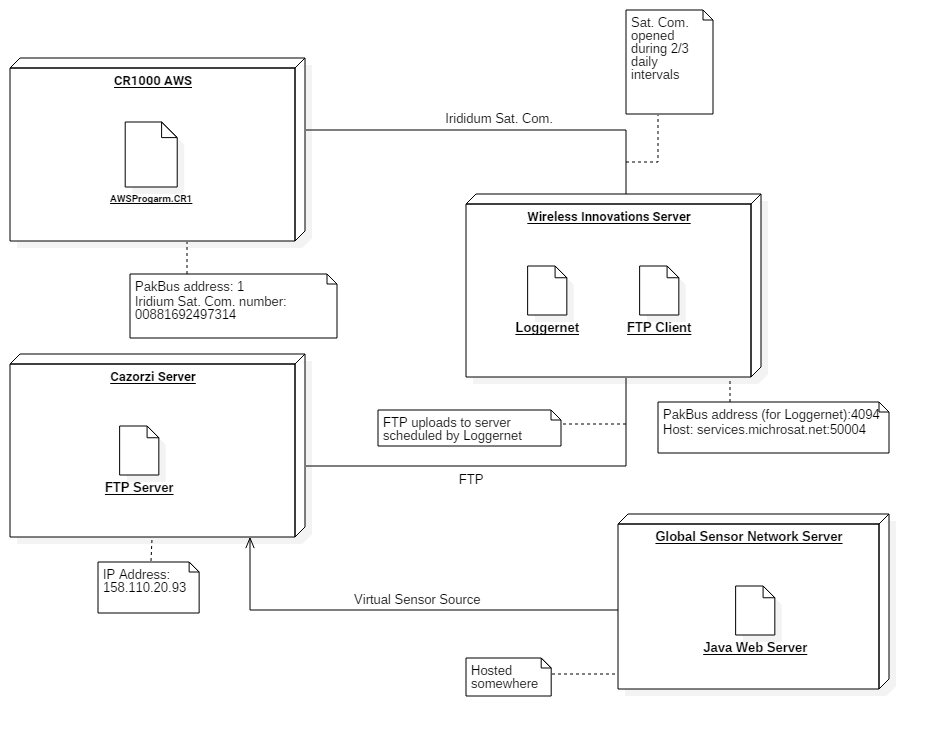
\includegraphics[width=\textwidth]{deployment_gns}
	\caption{Deployment UML diagram}
	\label{fig:depdiag}
\end{figure}